\chapter{Literature Review}

\section{Related works}

\subsection{Google Translate}

Google Translate is a widely used real-time translation application that supports multiple input modalities, including text, voice, handwriting, and camera images. The system produces translated outputs in both text and speech formats, and in the case of camera input, translated text can be displayed directly over the captured image.

The translation component of Google Translate is based on Google's Neural Machine Translation (GNMT) system. GNMT employs a deep encoder–decoder architecture built using recurrent neural networks (RNNs) combined with attention mechanisms. This architecture enables the system to model long-range dependencies in sentences, capture complex grammatical structures across different languages, and produce more accurate translations. In later developments, Google incorporated transformer-based architectures to improve translation speed and efficiency.

The main components of the GNMT architecture include:

\begin{itemize}
    \item \textbf{Encoder–Decoder RNNs:} The encoder converts input words into continuous vector representations, while the decoder generates the translated sequence based on these representations.

    \item \textbf{Deep Neural Layers:} GNMT uses multiple stacked RNN layers (up to eight layers) to improve the model's ability to capture complex linguistic patterns and contextual relationships.

    \item \textbf{Attention Mechanism:} The attention mechanism connects the encoder and decoder, allowing the model to focus on relevant parts of the input sentence during translation and helping to mitigate the short-memory limitations of traditional RNN architectures.
\end{itemize}

 It integrates with OCR (for camera input), ASR (speech recognition), and TTS (speech synthesis), making Google Translate multimodal.

\begin{figure}[h]
    \centering
    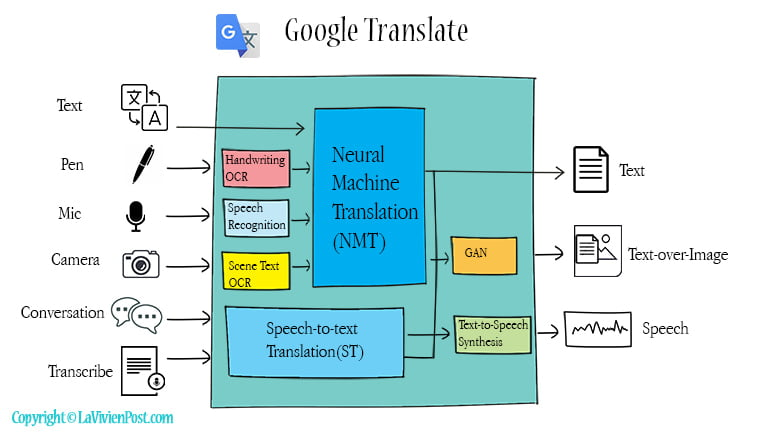
\includegraphics[width=\linewidth]{fig/google-translate.jpg}
    \caption{Architecture overview of Google Neural Machine Translation \cite{vivien2022gnmt}.}
    \label{fig:gnmt}
\end{figure}

\section{Current Research on Individual Components}

\subsection{OCR in Natural Scenes}

Optical Character Recognition (OCR) is widely used to convert printed or handwritten text into a digital form, enabling further processing such as search, editing, or translation \cite{liu2020scenetext}. In natural scene text recognition, the OCR task is typically divided into two stages: text detection and text recognition. The detection stage identifies regions of an image that contain text, while the recognition stage converts the detected text regions into character sequences.

Traditional OCR systems perform well when applied to structured documents with clean backgrounds and consistent fonts. However, scene text recognition presents additional challenges due to variations in lighting conditions, background complexity, perspective distortion, and font diversity \cite{szankin2025seeing}. To address these challenges, modern approaches often rely on deep learning-based models trained on large datasets of natural images.

Recent models such as Ocean-OCR improve robustness by increasing training data scale and model complexity, allowing the system to better handle noisy environments and diverse text styles \cite{chen2025oceanocr}. However, these large models typically require substantial computational resources and introduce higher inference latency. Such approaches are therefore less suitable for real-time mobile applications where computational efficiency is a critical constraint. As a result, lightweight OCR systems that prioritize speed and on-device inference are often used in mobile translation applications, even if this may slightly reduce recognition accuracy in challenging conditions \cite{bagal_2022image_translation}.

\subsection{Language Detection Techniques}

Language detection refers to the process of automatically identifying the language of a given text segment \cite{lui2014automatic}. This capability is important in multilingual translation systems because it allows the system to determine the source language before performing translation.

Two commonly used approaches for language detection are statistical n-gram methods and neural network–based approaches. N-gram methods analyze short character sequences within a text and estimate the probability that the text belongs to a particular language. These methods are computationally efficient and work well for short text segments, making them suitable for mobile applications.

Deep learning approaches, on the other hand, use neural networks to model more complex linguistic patterns and typically achieve higher accuracy \cite{gothe2020language}. However, such models often require greater computational resources and may introduce additional latency during inference. In mobile environments where computational efficiency is important, lightweight detection methods are often preferred.

\subsection{Machine Translation}

Machine translation (MT) is a fundamental task in natural language processing that aims to automatically convert text from one language to another \cite{tsujii1986future}. Early machine translation systems relied on rule-based or statistical approaches, but recent advances have been driven by neural machine translation (NMT).

Neural machine translation models typically employ encoder–decoder architectures that map input sentences into continuous vector representations and generate translated outputs based on these representations. The introduction of attention mechanisms further improved translation performance by allowing the model to focus on relevant parts of the input sentence during decoding.

More recently, transformer-based architectures have become the dominant approach for machine translation, offering improved scalability and parallelization compared to earlier recurrent neural network models \cite{kocmi2022findings}. These advances have significantly improved translation quality and enabled practical applications such as real-time multilingual translation systems.

For mobile translation applications, lightweight on-device translation models are commonly used to balance translation quality with computational efficiency. These models allow translation to be performed locally on the device without requiring continuous network connectivity.

\subsection{Scene Text Editing and Replacement}

Scene text editing refers to the task of modifying text that appears within natural images while preserving the surrounding visual context \cite{wu2019editing}. This problem lies at the intersection of computer vision, image synthesis, and text rendering. The objective is to replace the original text in an image with new content while maintaining consistency with the background, spatial layout, and visual appearance of the scene.

Early approaches to scene text editing often relied on generative adversarial networks (GANs) to jointly model background reconstruction and text generation \cite{wu2019editing}. These methods attempted to generate new text directly within the image while maintaining realistic visual integration with the surrounding scene.

More recent work has explored improved techniques for preserving text structure, font style, and alignment. For example, recognition-aware editing methods incorporate text recognition information to ensure semantic consistency between the generated text and the intended content \cite{fang2025rsste}. Other approaches such as the FASTER framework focus on preserving font appearance and spatial alignment while replacing text content \cite{das2025faster}.

Although these advanced models produce visually convincing results, many of them are computationally expensive and difficult to deploy in real-time mobile applications. For practical mobile systems, simpler techniques such as image inpainting combined with text re-rendering are often used to remove the original text region and insert translated text in a visually coherent manner.